\documentclass[aspectratio=169]{beamer}
% 
% Choose how your presentation looks.
% 
% For more themes, color themes and font themes, see:
% http://deic.uab.es/~iblanes/beamer_gallery/index_by_theme.html
% 
\mode<presentation>
{
  \usetheme{default}      % or try Darmstadt, Madrid, Warsaw, ...
  \usecolortheme{default} % or try albatross, beaver, crane, ...
  \usefonttheme{default}  % or try serif, structurebold, ...
  \setbeamertemplate{navigation symbols}{}
  \setbeamertemplate{caption}[numbered]
} 

\usepackage[english]{babel}
\usepackage[export]{adjustbox}
% \usepackage[utf8x]{inputenc}
\usepackage[style=authoryear]{biblatex}
\addbibresource{references.bib}
\usepackage{tikz}
\usepackage{xcolor}
\usepackage{relsize}
\usepackage{textcomp}
\usepackage[absolute,overlay]{textpos}
\graphicspath{{figures/}}
\DeclareMathOperator{\sign}{sign}
\usepackage{caption}
\captionsetup{font=scriptsize, labelfont=scriptsize}

\newcommand{\specialcell}[2][c]{%
  \begin{tabular}[#1]{@{}c@{}}#2\end{tabular}}

\title[Your Short Title]{When does vapor pressure deficit drive or reduce evapotranspiration?}
\author{Adam Massmann,  Pierre Gentine and Changjie Lin}
\institute{AGU Fall Meeting}
\date{December 14th, 2017}
\titlegraphic{\vspace*{1.0cm}\hspace*{-0.5cm}\includegraphics[width=6.0cm]{cu_logo.pdf}\hspace*{6.00cm}~%
   \includegraphics[width=1.5cm]{nsf.png}
}


\begin{document}

\begin{frame}
  \titlepage
\end{frame}


\section{Introduction}


\begin{frame}{Does VPD drive or reduce ET? - atmospheric demand perspective}
  \begin{columns}
    \begin{column}{0.7\textwidth}
      Increase in VPD (\textbf{increase in atmospheric demand}) drives  an \textbf{increase in ET}.
      \[VPD = (1-RH)\cdot e_s (T)\]
    \end{column}
    \begin{column}{0.3\textwidth}<2>      
      \includegraphics[width=\textwidth]{towel.jpg}
    \end{column}
  \end{columns}
\end{frame}

\begin{frame}{Does VPD drive or reduce ET? - plant response perspective}
  \begin{columns}
    \begin{column}{0.5\textwidth}
      However, plants evolved to use stomata to conserve and regulate water use. So \textbf{stomata closure} in response to increases in VPD may \textbf{decrease ET}.
    \end{column}
    \begin{column}{0.5\textwidth}
      \begin{figure}
        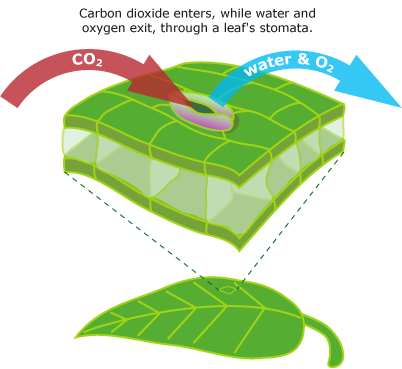
\includegraphics[width=2.25in]{stomata.png}% was O(1.5in)
        \caption{from evolution.berkeley.edu}
      \end{figure}
    \end{column}
  \end{columns}
\end{frame}


\begin{frame}{The question is, which effect dominates with an increase in VPD: plant response (decrease in ET) or atmospheric demand (increase in ET)?}
  \begin{itemize}
  \item Prior expectation:
    \begin{itemize}
    \item Should be a function of plant type: plants that are evolved to conserve water will tend to reduce ET with increases in VPD.
    \item But the environment still matters: if the atmosphere dries enough, plant water conservation strategies will reach their limit and atmospheric demand will drive increases in ET with increases in VPD.
    \end{itemize}
  \end{itemize}
\end{frame}

\section{Method}
\begin{frame}{Develop a theory to quantify ET response to VPD}
  \begin{itemize}
  \item The goal is to simply the problem (increase transparency) while still capturing the leading order behavior the system.
    \begin{itemize}
    \item Simplifying the system aids intrinsic understanding, but at a physical realism cost.
    \end{itemize}
  \item Because we run the risk of over-simplification, we will use FLUXNET2015 data to test how well our theory matches the data.
    \begin{itemize}
    \item We will test in the growing season of 5 plant types: deciduous broadleaf forest, evergreen needleleaf forest, shrub, grass, and crops.
    \end{itemize}
  \end{itemize}
\end{frame}

\begin{frame}{Simple theory - start with Penman-Monteith}
  We can use Penman-Monteith (PM) to estimate ET:
  \[ET = \frac{\Delta R + g_a \rho_a c_p \, VPD}{\Delta + \gamma(1 + \frac{g_a}{\textcolor{magenta}{\boldsymbol{g_s}}})},\]
  % \begin{overprint}
  %   \onslide<2>
    \textbf{Problem}: \Large $\textcolor{magenta}{\boldsymbol{g_s}}$ \normalsize (stomatal conductance) is a function of photosynthesis, which is a function of ET itself.  So ET in Penman-Monteith is really an implicit function of itself and we cannot take derivatives!
  % \end{overprint}
\end{frame}

\begin{frame}{Use physically reasonable assumptions remove implicit dependence}
  Apply a constant uWUE assumption (conserved within plant type; see \cite{Zhou_2016}):
  \[uWUE = \frac{GPP \cdot \sqrt{VPD}}{ET},\]
  \begin{overprint}
    \onslide<2>
    To derive a new form of Penman-Monteith without implicit ET dependence:
    \[  ET = \frac{\Delta R + \frac{g_a\; P}{T} \left( \frac{ c_p \, VPD}{R_{air}} -  \frac{\gamma c_s \sqrt{VPD} }{ R* \; 1.6 \text{ uWUE } (1 + \frac{g_1}{\sqrt{VPD}})} \right)}{ \Delta + \gamma}\]
    \end{overprint}
\end{frame}

\begin{frame}{Now just take $\frac{\partial \; ET}{\partial \; VPD}$}
  With our new form of Penman-Monteith we can now take derivatives, giving:
  \[\frac{\partial \;  ET}{\partial \, VPD} = \frac{2 g_a \; P}{T(\Delta + \gamma)}   \left(\frac{ c_p}{R_{air}} - \frac{\gamma c_s }{1.6 \; R*\; \text{ uWUE }} \left( \frac{2 g_1 + \sqrt{VPD}}{2 (g_1 + \sqrt{VPD})^2}\right) \right)\]
  In the interest of time, we will just focus in the ``sign'' term:
  \[\sign \left[\frac{\partial \;  ET}{\partial \, VPD}\right] = \sign \left[  \left(\frac{ c_p}{R_{air}} - \frac{\gamma c_s }{1.6 \; R*\; \text{ uWUE }} \left( \frac{2 g_1 + \sqrt{VPD}}{2 (g_1 + \sqrt{VPD})^2}\right) \right) \right] \]

\end{frame}

\section{Results - theory}
\begin{frame}{Consequences of theory - ``sign'' term}
  \begin{overprint}
    \onslide<1>
    \[\frac{\partial \, ET}{\partial \, VPD} = \text{scaling} \cdot \left(\frac{\textcolor{magenta}{\boldsymbol{ c_p}}}{R_{air}} - \frac{\gamma c_s }{1.6 \; \textcolor{magenta}{\boldsymbol{R*}}\; \text{ uWUE }} \left( \frac{2 g_1 + \sqrt{VPD}}{2 (g_1 + \sqrt{VPD})^2}\right) \right)\]
    \begin{itemize}
    \item $\textcolor{magenta}{\boldsymbol{c_p}}$ and $\textcolor{magenta}{\boldsymbol{R*}}$ are constants
    \end{itemize}
    \onslide<2>
    \[\frac{\partial \, ET}{\partial \, VPD} = \text{scaling} \cdot \left(\frac{ c_p}{\textcolor{magenta}{\boldsymbol{R_{air}}}} - \frac{\textcolor{magenta}{\boldsymbol{\gamma c_s}} }{1.6 \; R*\; \text{ uWUE }} \left( \frac{2 g_1 + \sqrt{VPD}}{2 (g_1 + \sqrt{VPD})^2}\right) \right)\]
    \begin{itemize}
    \item $c_p$ and $R*$ are constants
    \item $\textcolor{magenta}{\boldsymbol{R_{air}}}$, $\textcolor{magenta}{\boldsymbol{\gamma}}$, and $\textcolor{magenta}{\boldsymbol{c_s}}$ are approximately constant (relative to $\sqrt{VPD}$)
    \end{itemize}
    \onslide<3>
    \[\frac{\partial \, ET}{\partial \, VPD} = \text{scaling} \cdot \left(\frac{ c_p}{R_{air}} - \frac{\gamma c_s }{1.6 \; R*\; \text{ \textcolor{magenta}{\textbf{ uWUE}} }} \left( \frac{2  \textcolor{magenta}{\boldsymbol{g_1}} + \sqrt{VPD}}{2 ( \textcolor{magenta}{\boldsymbol{g_1}} + \sqrt{VPD})^2}\right) \right)\]

    \begin{itemize}
    \item $c_p$ and $R*$ are constants
    \item $R_{air}$, $\gamma$, and $c_s$ are approximately constant (relative to $\sqrt{VPD}$)
    \item \textcolor{magenta}{\textbf{uWUE}} and $\textcolor{magenta}{\boldsymbol{g1}}$ are constants within plant type.
    \end{itemize}
    \onslide<4>
    \[\frac{\partial \, ET}{\partial \, VPD} = \text{scaling} \cdot \left(\frac{ c_p}{R_{air}} - \frac{\gamma c_s }{1.6 \; R*\; \text{ uWUE }} \left( \frac{2 g_1 + \sqrt{VPD}}{2 (g_1 + \sqrt{VPD})^2}\right) \right)\]

    \begin{itemize}
    \item $c_p$ and $R*$ are constants
    \item $R_{air}$, $\gamma$, and $c_s$ are approximately constant (relative to $\sqrt{VPD}$)
    \item uWUE and $g1$ are constants within plant type
    \end{itemize}
    So \textbf{within each plant type}, whether the atmospheric demand (ET increasing with VPD) or plant response (ET decreasing with VPD) dominates is approximately \textbf{just a function of VPD}!
  \end{overprint}    
\end{frame}

\begin{frame}{``Sign'' term as a function of VPD and PFT}
  \begin{figure}
    \begin{tikzpicture}
      \node[anchor=south west,inner sep=0] (image) at (0,0) {\adjincludegraphics[width=3.3in, trim={0 {0.51\height} 0 0}, clip]{fig05.pdf}};
      \begin{scope}[x={(image.south east)},y={(image.north west)}]
        %% next four lines will help you to locate the point needed by forming a grid. comment these four lines in the final picture.↓
        % \draw[help lines,xstep=.1,ystep=.1] (0,0) grid (1,1);
        % \draw[help lines,xstep=.05,ystep=.05] (0,0) grid (1,1);
        % \foreach \x in {0,1,...,9} { \node [anchor=north] at (\x/10,0) {0.\x}; }
        % \foreach \y in {0,1,...,9} { \node [anchor=east] at (0,\y/10) {0.\y};}
        %% upto here
        \draw[-latex, line width=2pt] (0.83,0.725) --++(0.0in,0.3in)node[anchor=south] {ET Increasing};
        \draw[-latex, line width=2pt] (0.83,0.725) --++(0.0in,-0.3in)node[anchor=north] {ET Decreasing};

        % \draw[dashed,-latex, line width=5pt] (0.8,0.75) --++(0.0in,+0.5in)node[anchor=north] {ET Decreasing};
      \end{scope}
      % \node[align=center,red,font={\large}] at (image.southwest) {ET decreasing};
    \end{tikzpicture}
  \end{figure}
\end{frame}


\begin{frame}{``Sign'' term as a function of VPD and plant type}
  \begin{figure}
    \begin{tikzpicture}
      \node[anchor=south west,inner sep=0] (image) at (0,0) {\adjincludegraphics[width=3.3in, trim={0 {0.51\height} 0 0}, clip]{fig05_pet.pdf}};
      \begin{scope}[x={(image.south east)},y={(image.north west)}]
        %% next four lines will help you to locate the point needed by forming a grid. comment these four lines in the final picture.↓
        % \draw[help lines,xstep=.1,ystep=.1] (0,0) grid (1,1);
        % \draw[help lines,xstep=.05,ystep=.05] (0,0) grid (1,1);
        % \foreach \x in {0,1,...,9} { \node [anchor=north] at (\x/10,0) {0.\x}; }
        % \foreach \y in {0,1,...,9} { \node [anchor=east] at (0,\y/10) {0.\y};}
        %% upto here
        % \draw[-latex, line width=2pt] (0.83,0.725) --++(0.0in,0.3in)node[anchor=south] {ET Increasing};
        % \draw[-latex, line width=2pt] (0.83,0.725) --++(0.0in,-0.3in)node[anchor=north] {ET Decreasing};
        % \draw[dashed,-latex, line width=5pt] (0.8,0.75) --++(0.0in,+0.5in)node[anchor=north] {ET Decreasing};
      \end{scope}
      % \node[align=center,red,font={\large}] at (image.southwest) {ET decreasing};
    \end{tikzpicture}
  \end{figure}
  \begin{textblock*}{0.25\textwidth}(0.02\textwidth,0.3\textheight)
    \textcolor{magenta}{Dashed line} gives response for potential evapotranspiration (PET).\\
    \medskip
    Plants are crucial for land response!
  \end{textblock*}
\end{frame}


\section{Test Theory}
\begin{frame}{The theory seems nice, but we need to test with data!}
  Introduce a free uncertainty parameter \Large $\textcolor{magenta}{\boldsymbol{\sigma}}$ \normalsize to Penman Monteith:
  \[ET = \frac{\Delta R + \frac{g_a\; P}{T} \left( \frac{ c_p VPD}{R_{air}} -  \frac{\gamma c_s \sqrt{VPD} }{ R* \; 1.6\; \textcolor{magenta}{\boldsymbol{\mathlarger{\mathlarger{\sigma}}}} \; \text{ uWUE } (1 + \frac{g_1}{\sqrt{VPD}})} \right) }{ \Delta + \gamma}\]
  At each observation from FLUXNET (56 sites) calculate a unique \Large $\textcolor{magenta}{\boldsymbol{\sigma}}$ \normalsize:
  \[\textcolor{magenta}{\boldsymbol{\mathlarger{\sigma}}}(t, \text{site}) = f(ET_{obs})\]

  Then propagate uncertainty forward by including \Large $\textcolor{magenta}{\boldsymbol{\sigma}}$ \normalsize in the derivative:

  \[\frac{\partial \;  ET}{\partial \; VPD} = \text{scaling} \cdot \left(\frac{ c_p}{R_{air}} -  \frac{\gamma c_s }{1.6 \; R*\; \textcolor{magenta}{\boldsymbol{\mathlarger{\mathlarger{\sigma}}}} \; \text{ uWUE }} \left( \frac{2 g_1 + \sqrt{VPD}}{2 (g_1 + \sqrt{VPD})^2}\right) \right)\]
\end{frame}

\begin{frame}{Test theory with FLUXNET data - the good}
  \begin{textblock*}{1.0\textwidth}(0.3\textwidth,0.8\textheight)
    \textcolor{blue}{Blue line} is theory.\\
  \end{textblock*}

  \begin{columns}
    \begin{column}{0.33\textwidth}<1-3>
      \includegraphics[width=1.1\textwidth]{DBF_box.pdf}
    \end{column}
    \begin{column}{0.33\textwidth}<2-3>
      \includegraphics[width=1.1\textwidth]{CSH_box.pdf}
    \end{column}
    \begin{column}{0.33\textwidth}<3>
      \includegraphics[width=1.1\textwidth]{ENF_box.pdf}
    \end{column}
  \end{columns}
\end{frame}



\begin{frame}{Test theory with FLUXNET data - the bad}
  \begin{columns}
    \begin{column}{0.5\textwidth}
      \includegraphics[width=\textwidth]{GRA_box.pdf}
    \end{column}
    \begin{column}{0.5\textwidth}
      \includegraphics[width=\textwidth]{CRO_box.pdf}
    \end{column}
  \end{columns}
  \begin{textblock*}{1.0\textwidth}(0.3\textwidth,0.85\textheight)
    \textcolor{blue}{Blue line} is theory.\\
  \end{textblock*}

\end{frame}



% \begin{frame}{Summary of theory}
%   \begin{itemize}
%   \item We use \cite{Zhou_2016}'s uWUE to derive a new analytically tractable form of PM.
%   \item This new analysis suggests that the ``tipping'' point for which atmospheric demand overwhelms plant response will be almost exclusively a function of VPD.
%     \begin{itemize}
%     \item For each PFT there will be a VPD$_{crit}$ above which atmospheric demand will dominate and ET will increase with VPD.
%     \end{itemize}
%   \item Plant types evolved to conserve water (CSH) have a higher VPD$_{crit}$ than plants evolved (or bred) to use water and prioritize GPP (CRO). Trees and grasslands are somewhere between these two extremes.
%   \item Aerodynamic conductance scales the response, so plants with large surface roughness will be more likely to have a larger response as there is less resistance between the surface and the atmosphere.
%   \end{itemize}
% \end{frame}


\section{Conclusions}
% \begin{frame}{Summary}
%   \begin{itemize}
%   \item Theory finds that the ``tipping'' point for which atmospheric demand overwhelms plant response will be almost exclusively a function of VPD.  Plant types evolved to conserve water (CSH) have a higher VPD$_{crit}$ (and more negative ET response) than plants evolved (or bred) to use water and prioritize GPP (CRO).
%   \item On average, ecosystem response to VPD follows roughly what we might expect: CRO (prioritize GPP) has positive ET response to VPD, while all others have a negative response. Ordering by increasing magnitude of negative response gives: DBF, GRA, ENF, CSH; which roughly correspond to expectations for increasing water conservation as a function of PFT.
%   \item Uncertainty is high, especially for CRO and GRA. However, inclusion of uncertainty does not change the story for ENF or CSH.
%   \end{itemize}
% \end{frame}


\begin{frame}{Summary - When does VPD drive or reduce ET?}
  \begin{itemize}
  \item Theory predicts that each plant type has a \textbf{critical VPD} \textbf{below which ET will decrease} (plant response dominates), and \textbf{above which ET will increase} (atmospheric demand dominates).
  \item For forest sites, environmental VPD approximately straddles the critical VPD.
  \item For shrubs environmental VPD never exceeds the critical VPD.
  \item Theory tested poorly with FLUXNET data for for crops and grass. 
  \item All plant types exhibited a response far below that of PET.
  \item The new uWUE-version of Penman-Monteith we derived could be used as a complement for PET in drought indices over vegetated surfaces.
  \end{itemize}
\end{frame}

\section{References}
\begin{frame}{Acknowledgments - Thank you NSF and FLUXNET!!!}
  This work used eddy covariance data acquired and shared by the FLUXNET community, including these networks: AmeriFlux, AfriFlux, AsiaFlux, CarboAfrica, CarboEuropeIP, CarboItaly, CarboMont, ChinaFlux, Fluxnet-Canada, GreenGrass, ICOS, KoFlux, LBA, NECC, OzFlux-TERN, TCOS-Siberia, and USCCC. The ERA-Interim reanalysis data are provided by ECMWF and processed by LSCE. The FLUXNET eddy covariance data processing and harmonization was carried out by the European Fluxes Database Cluster, AmeriFlux Management Project, and Fluxdata project of FLUXNET, with the support of CDIAC and ICOS Ecosystem Thematic Center, and the OzFlux, ChinaFlux and AsiaFlux offices.\\
  \medskip
  This material is based upon work supported by the National Science Foundation Graduate Research Fellowship under Grant No. DGE 16-44869. Any opinion, findings, and conclusions or recommendations expressed in this material are those of the authors(s) and do not necessarily reflect the views of the National Science Foundation.
\end{frame}

\begin{frame}{References}
  \begin{enumerate}
  \item Franks, P. J., Berry, J. A., Lombardozzi, D. L., \& Bonan, G. B. (2017). Stomatal function across temporal and spatial scales: deep-time trends, land-atmosphere coupling and global models. \textit{Plant Physiology}, 174(2), 583-602.
  \item Lin, Y. S., Medlyn, B. E., Duursma, R. A., Prentice, I. C., Wang, H., Baig, S., ... \& De Beeck, M. O. (2015). Optimal stomatal behaviour around the world. Nature Climate Change, 5(5), 459-464.
  \item Medlyn, B. E., Duursma, R. A., Eamus, D., Ellsworth, D. S., Prentice, I. C., Barton, C. V., ... \& Wingate, L. (2011). Reconciling the optimal and empirical approaches to modelling stomatal conductance. \textit{Global Change Biology}, 17(6), 2134-2144.
  \item Zhou, S., Yu, B., Huang, Y., \& Wang, G. (2015). Daily underlying water use efficiency for AmeriFlux sites. \textit{Journal of Geophysical Research: Biogeosciences}, 120(5), 887-902.
  \end{enumerate}
\end{frame}

\begin{frame}{Summary - When does VPD drive or reduce ET?}
  \begin{itemize}
  \item Theory predicts that each plant type has a \textbf{critical VPD} \textbf{below which ET will decrease} (plant response dominates), and \textbf{above which ET will increase} (atmospheric demand dominates).
  \item For forest sites, environmental VPD approximately straddles the critical VPD.
  \item For shrubs environmental VPD never exceeds the critical VPD.
  \item Theory tested poorly with FLUXNET data for for crops and grass. 
  \item All plant types exhibited a response far below that of PET.
  \item The new uWUE-version of Penman-Monteith we derived could be used as a complement for PET in drought indices over vegetated surfaces.
  \end{itemize}
  \bigskip
  \medskip
  Adam Massmann:\textbf{ akm2203@columbia.edu }
\end{frame}

% \section{Extra Slides}

% \begin{frame}{Extra slide - statistics}
%   \begin{table}
%     \label{vpd_crit}
%     \caption{More quantitative test of theory.}
%     \centering
%     \begin{tabular}{l c c c c c c}
%       \hline
%       PFT & \specialcell{Fraction of Obs.\\Theory is Correct} & Mean ($\frac{\partial \; ET}{\partial \; VPD} < 0$) & Mean ($\frac{\partial \; ET}{\partial \; VPD} > 0$)\\
%       \hline
%       CRO & 0.566517 & -0.209152 &  0.005856\\
%       CSH & 0.931660 & -0.264746 &       NaN\\
%       DBF & 0.633363 & -0.135679 &  0.042910\\
%       ENF & 0.633138 & -0.150665 &  0.029281\\
%       GRA & 0.442306 & -0.042158 & -0.042480\\
%       \hline
%     \end{tabular}
%   \end{table}
% \end{frame}

% \begin{frame}{Quantitative $VPD_{crit}$}

%   \scriptsize
%   \begin{table}
%     \label{vpd_crit}
%     \caption{Values of $VPD_{crit}$, where $\frac{\partial \; ET}{\partial \; VPD} = 0$, evaluated at PFT average values for $R_{air}$, $\sigma$, $\gamma$, and $c_s$. For reference, these values are also provided. For values of $VPD$ less than $VPD_{crit}$, $\frac{\partial \; ET}{\partial \; VPD}$ will be negative, and for values of $VPD$ greater than $VPD_{crit}$, $\frac{\partial \; ET}{\partial \; VPD}$ will be positive.}
%     \centering
%     \begin{tabular}{l c c c c c}
%       \hline
%       PFT & $R_{air}$ & $c_s$ (ppm) & $\gamma$ &  uWUE & \textbf{$VPD_{crit}$ (Pa)} \\
%       \hline
%       CRO &  288.680920 & 372.567691& 65.351523& 2.602873&  \textbf{133.165438} \\
%       CSH &   289.067152& 381.593622& 67.613172& 2.175278& \textbf{4439.564212} \\
%       DBF &   288.624437& 377.449849& 63.421812& 2.746393&  \textbf{888.773243} \\
%       ENF &  288.183849& 377.676463& 61.559242& 4.015362&  \textbf{978.084845} \\
%       GRA &  288.425651& 377.264645& 61.598768& 2.281074& \textbf{1141.630778} \\
%       \hline
%       \multicolumn{2}{l}{}
%     \end{tabular}
%   \end{table}
% \end{frame}

% \begin{frame}{Statistics with uncertainty}
%   \scriptsize
%   \begin{table}
%     \caption{Statistics of $\frac{\partial \; ET}{\partial \; VPD}$ as a function of PFT.}
%     \centering
%     \begin{tabular}{l c c c c c}
%       \hline
%       PFT & $\overline{\frac{\partial \; ET}{\partial \; VPD}}$ & $\frac{\partial \; ET}{\partial \; VPD}\left(\overline{env}\right)$ & $\frac{\partial \; ET}{\partial \; VPD}\left(\overline{env}\right)*\text{std}(VPD)$ & $\frac{\frac{\partial \; ET}{\partial \; VPD}\left(\overline{env}\right)*\text{std}(VPD)}{ \frac{\partial \; ET}{\partial \; R}\left(\overline{env}\right)*\text{std}(R)}$ & fraction $\frac{\partial \; ET}{\partial \; VPD} < 0.$ \\
%       \hline
%       CRO & 0.000853 & 0.026241 & 37.05 & 0.41 & 0.473311\\
%       CSH & -0.108234 & -0.091526 & 101.72 & 0.88 & 0.931660\\
%       DBF & -0.012727 & 0.013794 & 39.47 & 0.33 & 0.461674\\
%       ENF & -0.034087 & 0.000706 & 33.22 & 0.30 & 0.534425\\
%       GRA & -0.019637 & -0.000921 & 33.60 & 0.35 & 0.631735\\
%       \hline
%       \multicolumn{2}{l}{}

      
%     \end{tabular}
%   \end{table}
% \end{frame}

% \begin{frame}{Scaling Term}
%   \[\frac{\partial \;  ET}{\partial \; D} = \mathbf{ \frac{g_a \; P}{T(\Delta + \gamma)} }   \left(\frac{ c_p}{R_{air}} - \frac{\text{LAI$_{ref}$}}{\text{LAI}} \frac{\gamma c_s }{1.6 \; R*\; \text{ uWUE }} \left( \frac{2 g_1 + \sqrt{D}}{2 (g_1 + \sqrt{D})^2}\right) \right)\]
%   \begin{figure}
%     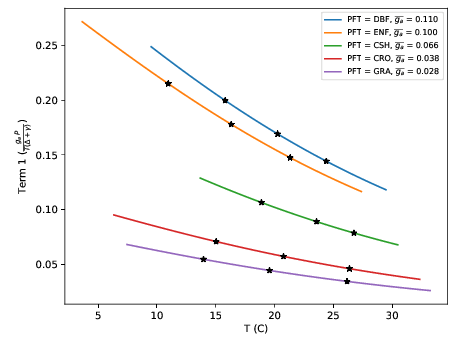
\includegraphics[width=3.0in]{scaling.png}
%     % \caption{}
%   \end{figure}
% \end{frame}


% \begin{frame}{Extra slide - is theory VPD$_{crit}$ optimum?}
%   \includegraphics[width=0.7\textwidth]{for_agu.pdf}
% \end{frame}

% \begin{frame}{Test theory with FLUXNET data - CSH}
%   \includegraphics[width=3.5in]{csh_eee.png}
% \end{frame}

% \begin{frame}{Test theory with FLUXNET data - ENF}
%   \includegraphics[width=3.5in]{enf_eee.png}
% \end{frame}


% \begin{frame}{Test theory with FLUXNET data - DBF}
%   \includegraphics[width=3.5in]{dbf_eee.png}
% \end{frame}

% \begin{frame}{Test theory with FLUXNET data - CRO}
%   \includegraphics[width=3.5in]{cro_eee.png}
% \end{frame}

% \begin{frame}{Test theory with FLUXNET data - GRA}
%   \includegraphics[width=3.5in]{gra_eee.png}
% \end{frame}

% \begin{frame}{Consequences of theory - ``sign'' term}
% Below is a little opaque (at least to me):
% \[\frac{\partial \, ET}{\partial \, VPD} = \text{scaling} \cdot  \left(\frac{ c_p}{R_{air}} - \frac{\gamma c_s }{1.6 \; R*\; \text{ uWUE }} \left( \frac{2 g_1 + \sqrt{VPD}}{2 (g_1 + \sqrt{VPD})^2}\right) \right)\]
% so do expansion about $g_1 >> \sqrt{VPD}$:
% \footnotesize
% \[ \frac{\partial \, ET}{\partial \, VPD} \approx \text{scaling} \cdot  \left(\frac{ c_p}{R_{air}} - \frac{\gamma c_s }{1.6 \; R*\; \text{ uWUE }} \left( \frac{1}{g_1} - \frac{3\sqrt{VPD}}{2 g_1^2} +  \mathcal{O}\left(\frac{\sqrt{VPD}}{g_1}\right)^{2} \right) \right)\]
% % \large
% % and:
% %   \[ \sqrt{VPD} \Big|_{\frac{\partial ET}{\partial VPD} = 0} \approx  \frac{2 g_1}{3}  \left( -\frac{ c_p \, g_1\,  1.6  \; R*\; \text{ uWUE }}{R_{air} \gamma c_s } + 1  \right) \]

% %   \[ VPD \Big|_{\frac{\partial ET}{\partial VPD} = 0} = \frac{R_{air}}{4 \, c_p} \left[ \frac{\gamma  c_s}{R* \, 1.6\, \text{uWUE}} + \sqrt{\left(g_1 + 8\, \frac{c_p}{R_{air}}\right) \frac{\gamma c_s}{R* \, 1.6\, \text{uWUE}}} - 4 \, g_1 \frac{ c_p}{R_{air}}\right] \]
% \end{frame}


% \begin{frame}{Is uncertainty a function of VPD?}
%   \includegraphics[width=3.0in]{vpd_sigma.png}
% \end{frame}

% \begin{frame}{How to take VPD derivative?}
%   % below gnereated in fig03.py
%   \includegraphics[width=3.0in]{e_s_rh.png}
% \end{frame}


% % \begin{frame}{Summary statistics - extra sl}
% %   \begin{table}
% %     \caption{Statistics of $\frac{\partial \; ET}{\partial \, VPD}$ as a function of PFT.}
% %     \centering
% %     \begin{tabular}{l c c}
% %       \hline
% %       PFT & $\overline{\frac{\partial \; ET}{\partial \; VPD}}$ & fraction $\frac{\partial \; ET}{\partial \; VPD} < 0.$ \\
% %       \hline
% %       CRO & 0.000853  & 0.473311\\
% %       CSH & -0.108234 & 0.931660\\
% %       DBF & -0.012727 & 0.461674\\
% %       ENF & -0.034087 & 0.534425\\
% %       GRA & -0.019637 & 0.631735\\
% %       \hline
% %       \multicolumn{2}{l}{}  
% %     \end{tabular}
% %   \end{table}
% % \end{frame}

% % \begin{table}
% %   \centering
% %   \begin{tabular}{l|r}
% %     Item & Quantity \\\hline
% %     Widgets & 42 \\
% %     Gadgets & 13
% %   \end{tabular}
% %   \caption{\label{tab:widgets}An example table.}
% % \end{table}

\end{document}
